% \documentclass{book}

\documentclass[12pt]{article}
\usepackage[pdfborder={0 0 0.5 [3 2]}]{hyperref}%
\usepackage[left=1in,right=1in,top=1in,bottom=1in]{geometry}%
\usepackage[shortalphabetic]{amsrefs}%
\usepackage{amsmath}
\usepackage{enumerate}
\usepackage{enumitem}
\usepackage{amssymb}                
\usepackage{amsmath}                
\usepackage{amsfonts}
\usepackage{amsthm}
\usepackage{bbm}
\usepackage[table,xcdraw]{xcolor}
\usepackage{tikz}
\usepackage{float}
\usepackage{svg}
\usepackage{mathtools}
\usepackage{cool}
\usepackage{url}
\usepackage{graphicx,epsfig}
\usepackage{makecell}
\usepackage{array}

\graphicspath{ {images/} }
\renewcommand{\arraystretch}{3}

\begin{document}

\title{}
\author{\vspace{-10ex} }

\begin{center}
{\LARGE APMA 1650 -- Midterm 1}\\
\vspace{5mm}
{\large Wednesday, July 13, 2016 }\\
\vspace{10mm}
{\large Name: }
\vspace{3cm}

\begin{figure}[H]
\centering
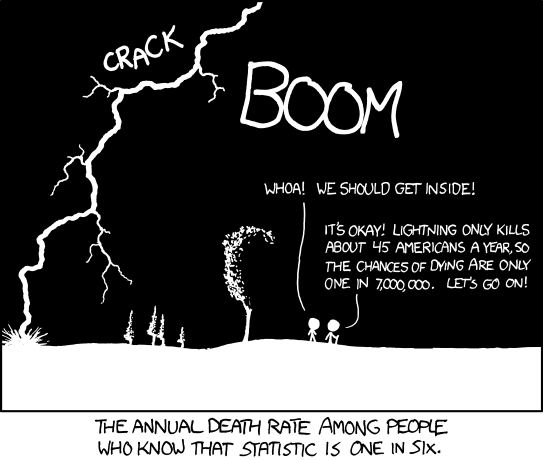
\includegraphics[width=15cm]{xkcd1}
\end{figure}
% {\large Due Tuesday, July 5, 2016}\\
% \vspace{5mm}
\end{center}
\pagebreak

\begin{center}
{\LARGE Instructions}\\
\vspace{5mm}
\end{center}

\begin{itemize}
\item The exams begins at 1:00 pm and ends at 3:00 pm. You have 2 hours to complete the exam.
\item You may use a calculator if you wish (although the exam is designed to be done without one, so I am not sure how helpful one will be). Other electronic devices may not be used and must be stowed beneath the seat in front of you or in the overhead compartment for the duration of the exam. You may not use any books or notes. 
\item Write all answers in the space below the question. If you need more space, feel free to use the back of the page.
\item Correct expressions are sufficient. You do not need to simplify your answers. You can leave answers in terms of binomial coefficients such as $\binom{64}{5}$, exponents such as $(1/2)^{10}$ or $2^{16}$, and factorials such as $12!$.
\item There are 5 questions. Each question is worth 10 points. Partial credit will be given for partially correct answers.
\item Unless you have found an error on the exam, in the interest of fairness, the exam proctor will likely not answer any questions you have about the test.
\item All answers must be fully justified. Show all of your work. Points will be deducted for unjustified answers.
\item I recommend you look through the entire exam first before answering any questions. That way you can start with the questions you find to be easiest.
\item The list of the common probability distributions, together with their pmfs/densities, expected values, and variances, is attached to the back of the exam. A $Z$-table and a $t$-table is also included at the back of the exam.
\end{itemize}

\begin{figure}[H]
\centering
\label{my-label}
\begin{tabular}{|l|l|l|l|l|l|l|}
\hline
Problem & $\:\:1\:\:$ & $\:\:2\:\:$ & $\:\:3\:\:$ & $\:\:4\:\:$ & $\:\:5\:\:$ & Total \\ \hline
Points  &   &   &   &   &   &       \\ \hline
\end{tabular}
\end{figure}

\pagebreak

\begin{enumerate}
\item (10 points) 

\pagebreak

\item (10 points)

\pagebreak Let $Y$ be a Binomial r

\item (10 points) 

\pagebreak

\item 
\pagebreak

\item

\end{enumerate}

\pagebreak


\begin{figure}[H]
\caption{Discrete Distributions}
\begin{tabular}{l c c c c}
\hline
Distribution & Parameters & Probability Mass Function (pmf) & Mean & Variance \\
\hline
Binomial & $n, p$ & \makecell{ $\displaystyle p(y) = \binom{n}{y}p^y(1-p)^{n-y}$\\$ \displaystyle y = 0, 1, \dots, n$} & $np$ & $np(1-p)$ \\
Geometric & $p$ & \makecell{ $\displaystyle p(y) = (1-p)^{y-1}p$ \\ $y = 1, 2, \dots$} & $ \displaystyle \frac{1}{p}$ & $\displaystyle \frac{1 - p}{p^2}$ \\
Poisson & $\lambda$ & \makecell{ $\displaystyle p(y) = \frac{e^{-\lambda} \lambda^y }{y!}$ \\ $y = 0, 1, 2, \dots$ } & $\lambda$ & $\lambda$ \\
\end{tabular}
\end{figure}

\vspace{2cm}

\begin{figure}[H]
\caption{Continuous Distributions}
\begin{tabular}{l c c c c}
\hline
Distribution & Parameters & Probability Density Function (pdf) & Mean & Variance \\
\hline
Uniform & $a, b$ & \makecell{ $\displaystyle f(y) = \frac{1}{b-a}$ \\ $a \leq y \leq b$ }& $\displaystyle \frac{a + b}{2}$ & $\displaystyle \frac{(b - a)^2}{12}$ \\
Exponential & $\lambda$ & \makecell{ $\displaystyle f(y) = \lambda e^{-\lambda y}$ \\ $0 \leq y < \infty$} & $\displaystyle \frac{1}{\lambda}$ & $\displaystyle \frac{1}{\lambda^2}$ \\
Normal & $\mu, \sigma$ & $\displaystyle f(y) = \frac{1}{\sqrt{2 \pi}\sigma}e^{- \frac{(y - \mu)^2}{2 \sigma^2}}$ & $\mu$ & $\sigma^2$ \\
Standard Normal & none & $\displaystyle f(y) = \frac{1}{\sqrt{2 \pi}}e^{- \frac{y^2}{2}}$ & $0$ & $1$ \\
\end{tabular}
\end{figure}

\end{document}

